% !TEX TS-program = xelatex 
% !TEX encoding = UTF-8
\documentclass{article}

\usepackage{jcs-thesis-fonts}
\usepackage{jcs-thesis-punct}
\usepackage{jcs-thesis-dates}
\usepackage{jcs-thesis-bibidx}
\usepackage{jcs-thesis-theorem}
\usepackage{jcs-thesis-math}

\usepackage{tikz}
\usetikzlibrary{matrix,arrows}

\begin{document}
\title{Control Systems for the\\%
%	Northrop Grumman\\%
	Lunar Lander X-Prize Challenge\\%
	Interim Report \No 2:\\%
	Dynamic Programming}
\author{Joel C. Salomon}
\date{\today\\\currenttime}
\special{pdf: docinfo <<
	/Title		(Thesis Report 2: Dynamic Programming)
\ifxetex /Creator	(XɘLᴬTeX with hyperref package)\else\fi
	/Author		(Joel C. Salomon)
	/CreationDate	(D:20100514120000)
	/ModDate		(D:\pdfdate)
	/Subject		(Engineering)
	/Keywords		(control systems;optimal control;dynamic programming;rocket landing)
	>>}
%\cleardoublepage
\maketitle

\section*{Overview}
To recap from Interim Report \No~1,
the optimal control problem boils down to
finding a suitable control trajectory $\vecu$
which will cause the system,
itself describable by 
\begin{equation}
	\label{rpt:forml:eq:stateeq:vect}
	\tag{\textsc{r}1:1${}′$}
	\dot{\vecx}(t) =
		\func{\veca}{\vecx(t), \vecu(t), t}
\end{equation}
which will minimize the performance measure
\begin{equation}
	\label{rpt:forml:eq:measure}
	\tag{\textsc{r}1:2}
	J = \func{h}{\vecx(t_\fl),t_\fl} +
		\intt{\func{g}{\vecx(t), \vecu(t), t} \dd t}.
\end{equation}
(Equation numbers beginning with \textsc{r}$x$
refer to previous reports, so that
\eqref{rpt:forml:eq:stateeq:vect} and \eqref{rpt:forml:eq:measure}
refer to equations (1${}′$) and (2)
from \citetitle{salomon:report1}.)

This report will discuss the use of
\emph{dynamic programming} in optimization.
As before, the notation used in this report
largely follows Kirk’s \citetitle{kirk:optintro}.

\tableofcontents

\section{Admissibility}
In the previous report (§1.2) I simply mentioned that
“[t]here will often be constraints on the states or the control inputs”
and glossed over the issue of admissibility,
so a short digression in that direction is in order.

\begin{defn}
	Almost all real-life systems will have constraints,
	whether physical or regulatory.
	An \emph{admissible trajectory}
	is a state trajectory \( \vecx \) for which
	the state variable constraints on \( \vecx(t) \) are obeyed
	over the interval \( [t_\il, t_\fl] \);
	let \( X \) denote the set of such admissible trajectories.
	\par
	Similarly, an \emph{admissible control}
	is a control curve \( \vecu \) for which
	the control constraints on \( \vecu(t) \) are obeyed
	over the interval \( [t_\il, t_\fl] \),
	and which causes the state \( \vecx(t) \) to follow
	an admissible trajectory \( \vecx \in X \);
	let \( U \) denote the set of such admissible controls.
\end{defn}

The optimal control problem can now be written more precisely:
Find an \emph{admissible control} \( \vecu\opt \)
which causes the system
\[
	\dot{\vecx}(t) =
		\func{\veca}{\vecx(t), \vecu(t), t}
\]
to follow an \emph{admissible trajectory} \( \vecx \)
that minimizes the performance measure
\[
	J = \func{h}{\vecx(t_\fl),t_\fl} +
		\intt{\func{g}{\vecx(t), \vecu(t), t} \dd t};
\]
\( \vecu\opt \) is called an \emph{optimal control} and
\( \vecx\opt \) an \emph{optimal trajectory}.

\bigskip\noindent
We now begin the actual topic of this report,
which is finding a closed-loop
\emph{optimal control law}, or \emph{optimal policy},
\[
	\vecu\opt(t) = \func{\mathbf{f}}{\vecx(t), t)}
\]
via \emph{dynamic programming}.

\section{The Principle of Optimality}
Foo!
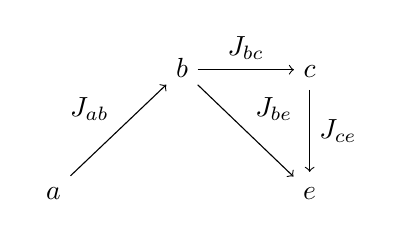
\begin{tikzpicture}[description/.style={fill=white, inner sep=2pt}]
	\matrix (m) [matrix of math nodes, row sep=3em,
		column sep=3.5em, text height=1.5ex, text depth=0.25ex]
	{   & b & c \\
	  a &   & e \\ };
	\path[->]
	(m-2-1) edge node[auto] {$J_{ab}$} (m-1-2)
	(m-1-2) edge node[auto] {$J_{be}$} (m-2-3)
	        edge node[auto] {$J_{bc}$} (m-1-3)
	(m-1-3) edge node[auto] {$J_{ce}$} (m-2-3);
\end{tikzpicture}

\section{Future Work}
The next Interim Report will focus on …

I am posting notes on my progress on my blog at
\url{http://optimalcontrol.wordpress.com/};
in-progress thesis work is in my publicly visible GitHub repository,
\url{http://github.com/jcsalomon/thesis}.

%\cleardoublepage
\printbibliography[heading=bibintoc]

\end{document}

